\documentclass[a4paper,UTF8]{article}
\usepackage{ctex}
\usepackage[margin=1.25in]{geometry}
\usepackage{color}
\usepackage{graphicx}
\usepackage{amssymb}
\usepackage{amsmath}
\usepackage{amsthm}
\usepackage{enumerate}
\usepackage{bm}
\usepackage{hyperref}
\usepackage{epsfig}
\usepackage{mdframed}
\usepackage{lipsum}
\usepackage{mathtools}
\usepackage{algorithm}
\usepackage{algorithmic}
\usepackage{diagbox}
\usepackage{booktabs}
\usepackage{multirow}
\newmdtheoremenv{thm-box}{myThm}
\newmdtheoremenv{prop-box}{Proposition}
\newmdtheoremenv{def-box}{定义}

\setlength{\evensidemargin}{.25in}
\setlength{\textwidth}{6in}
\setlength{\topmargin}{-0.5in}
\setlength{\topmargin}{-0.5in}
% \setlength{\textheight}{9.5in}
%%%%%%%%%%%%%%%%%%此处用于设置页眉页脚%%%%%%%%%%%%%%%%%%
\usepackage{fancyhdr}                                
\usepackage{lastpage}                                           
\usepackage{layout}                                             
\footskip = 10pt 
\pagestyle{fancy}                    % 设置页眉                 
\lhead{2018年秋季}                    
\chead{高级机器学习}                                                
% \rhead{第\thepage/\pageref{LastPage}页} 
\rhead{作业二}                                                                                               
\cfoot{\thepage}                                                
\renewcommand{\headrulewidth}{1pt}  			%页眉线宽,设为0可以去页眉线
\setlength{\skip\footins}{0.5cm}    			%脚注与正文的距离           
\renewcommand{\footrulewidth}{0pt}  			%页脚线宽,设为0可以去页脚线

\makeatletter 									%设置双线页眉                                        
\def\headrule{{\if@fancyplain\let\headrulewidth\plainheadrulewidth\fi%
\hrule\@height 1.0pt \@width\headwidth\vskip1pt	%上面线为1pt粗  
\hrule\@height 0.5pt\@width\headwidth  			%下面0.5pt粗            
\vskip-2\headrulewidth\vskip-1pt}      			%两条线的距离1pt        
 \vspace{6mm}}     								%双线与下面正文之间的垂直间距              
\makeatother  

%%%%%%%%%%%%%%%%%%%%%%%%%%%%%%%%%%%%%%%%%%%%%%
\numberwithin{equation}{section}
%\usepackage[thmmarks, amsmath, thref]{ntheorem}
\newtheorem{myThm}{myThm}
\newtheorem*{myDef}{Definition}
\newtheorem*{mySol}{Solution}
\newtheorem*{myProof}{Proof}
\newcommand{\indep}{\rotatebox[origin=c]{90}{$\models$}}
\newcommand*\diff{\mathop{}\!\mathrm{d}}

\usepackage{multirow}

%--

%--
\begin{document}
\graphicspath{{image/}}
\title{高级机器学习\\
作业二}
\author{brooksj}
\maketitle

\section{[30pts] Learning Theory}
\begin{enumerate}[(1)]
	\item \textbf{[10pts] VC维} 

	试讨论最近邻分类器假设空间的VC维大小,并给出证明.
	\item \textbf{[10pts] Rademaher复杂度}
	
	试证明: 常数函数$c$的Rademaher复杂度为$0$.
	\item \textbf{[10pts] PAC} 
	
	$\mathcal{X}=\mathbb{R}^2, \mathcal{Y}= {0,1}.$假设空间$\mathcal{H}$定义如下:$\mathcal{H}=\{h_r:r \in \mathbb{R}_+\}$,其中$h_r (x)=\mathbb{I}(\parallel x \parallel \leq r)$,假定假设空间是可分的,证明$\mathcal{H}$是PAC可学习的,并且样本复杂度为$\frac{log(1/\delta)}{\epsilon}$
	\newline
	(提示:可考虑返回与训练集一致的最小圆的算法)
\end{enumerate}
\begin{myProof}
此处用于写证明(中英文均可)\\\\
(1)最近邻分类器的Rademachar复杂度为无穷大。\\
证:最近邻分类器的模型由训练集样本决定,可以通过构建训练样本来构建一个分类器。对于任意数量为m的样本集合D中的每一个样本$x_i$,它的最近邻距离为$d=\min_{x_j \in D \backslash x_i}dist(x_i,\ x_j)$,在样本附近放置1个训练样本$x_i^{'}$满足$dist(x_i,\ x_i^{'})\ <\ d$,而最近样本点的类别决定了$x_i$的分类,于是样本分类有$2^m$种,因此最近邻分类器假设空间的VC维大小为无穷大。\\\\


\noindent
(2)证:由课本上chapter12的公式(12.40)可知常数函数c的Rademacher复杂度为
\begin{eqnarray*}
    \hat{R}_Z(\mathcal{F})\ &=&\ \mathbb{E}_\epsilon[\sup_{f \in \mathcal{F}}\frac{1}{m}\sum_{i=1}^m\sigma_if(z_i)]\\
    &=&\mathbb{E}_\epsilon[\frac{1}{m}\sum_{i=1}^m \sigma_i c]\\
    &=&\frac{c}{m}\sum_{i=1}^{m}\mathbb{E}(\sigma_i)
\end{eqnarray*}
又因为$\sigma_i$是随机变量,以0.5的概率取1,0.5的概率取-1,所以$\mathbb{E}(\sigma_i)=0$,由此可得
\begin{equation*}
    \hat{R}_Z(\mathcal{F})\ =\ \frac{c}{m}\sum_{i=1}^{m}\mathbb{E}(\sigma_i) = 0
\end{equation*}
同时由课本上chapter12的公式(12.41)可得:
\begin{equation*}
    R_m(\mathcal{F})\ =\ \mathbb{E}_{Z \subseteq \mathcal{Z}:|Z|=m}[\hat{R}_Z(\mathcal{F})]\ =\ 0
\end{equation*}
\\

\noindent
(3)证:引用一下PAC可学习的定义:令m表示从分布$\mathcal{D}$中独立同分布采样得到的样例数目,$0<\epsilon,\delta<1$,对所有分布$\mathcal{D}$,若存在学习算法$\mathcal{L}$和多项式$poly(.,.,.,.)$,使得对于任何$m \ge poly(1/\epsilon,1/\delta,size(\mathbf{x}),size(c))$,$\mathcal{L}$能从假设空间$\mathcal{H}$中PAC辨识概念类$\mathcal{C}$,则称概念类$\mathcal{C}$对假设空间$\mathcal{H}$而言是PAC可学习的。\\
本题中$size(x)=2,size(c)=1$,所以只需证明对于任意$m \ge poly(1/\epsilon,1/\delta)$,$\mathcal{L}$可从假设空间$\mathcal{H}$中PAC辨识概念类$\mathcal{C}$即证明
\begin{eqnarray}
    P(E(h) \le \epsilon) \ge 1-\delta
\end{eqnarray}
因为假设空间是可分的,所以目标概念存在于假设空间中,设目标概念c为$c(x)=\mathbb{I}(\left\|\ x\ \right\| \le r_c)$。目标算法为返回与训练集大小一致的最小圆算法,设r为训练集的正样本中离原点距离最远的距离,那么$r \le r_c$。\\
假设最终学得的最小圆算法半径为$r_\epsilon$,设点落在半径为$r_c$的圆和半径为$r_\epsilon$之间的概率为$\epsilon$,采样点在圆环内的概率为$\epsilon$,不在圆环内的概率为$1-\epsilon$,保证每次采样都是独立同分布的,则
\begin{eqnarray*}
    P(E(h)\ \le\ \epsilon)\ &=&\ P(min(r_\epsilon,\ r_c)\ \le\ r\ \le\ max(r_\epsilon,\ r_c))\\
    &=& 1\ -\ (1-\epsilon)^m\ >\ 1\ -\ e^{-m\epsilon}
\end{eqnarray*}
结合式(1.1)只需使$1\ -\ e^{-m\epsilon} >= 1 - \delta$,可得$m\ \ge\ \frac{ln(1/\delta)}{\epsilon}$,显然符合PAC可学习的定义,因此$\mathcal{H}$是PAC可学习的,并且样本复杂度为$\frac{ln(1/\delta)}{\epsilon}$。\\
证毕!


\end{myProof}
\newpage

\section{[30pts] 文档主题模型}
在一个新闻数据集上实现文档主题模型(Latent Dirichlet Allocation~(LDA))~\cite{DBLP:journals/jmlr/BleiNJ03}.

我们提供了一个包含8,888条新闻的数据集,请在该数据集上完成LDA算法的使用及实现。

\begin{itemize}
	\item 数据集下载:\href{http://lamda.nju.edu.cn/ml2018grad/dataset/news.txt.zip}{新闻数据集.}
	\item 格式:每行是一条新闻.
\end{itemize}

数据预处理提示:你可能需要完成分词及去掉一些停用词等预处理工作.

\begin{enumerate}[(1)]
	\item \textbf{[10pts] 任务\#1:使用LDA模型} 
	\subitem A. 选择开源的LDA库(例如:\href{https://scikit-learn.org/stable/modules/generated/sklearn.decomposition.LatentDirichletAllocation.html}{scikit-learn}),并在提供的数据集上学习使用.
	\subitem B. 给出$K=\{5,10,20\}$个主题时,每个主题下概率最大的$M=10$个词及其概率.
	\item \textbf{[20pts] 任务\#2:实现LDA模型} 
	\subitem A. 不借助开源库,自己完成LDA算法.
	\subitem B. 给出$K=\{5,10,20\}$个主题时,每个主题下概率最大的$M=10$个词及其概率.
\end{enumerate}
\begin{mySol}
\newpage
\noindent
(1)解:\\
k=5个主题时
\begin{table*}[htbp]
	\centering
	\newcommand{\tabincell}[2]{\begin{tabular}{@{}#1@{}}#2\end{tabular}}
    \caption{k = 5个主题时的结果(sklearn)}
    \begin{tabular}{c p{1.8cm}<{\centering} p{1.6cm}<{\centering} p{1.4cm}<{\centering} p{1.4cm}<{\centering} p{1.2cm}<{\centering} p{1.2cm}<{\centering} p{1.0cm}<{\centering} p{1.0cm}<{\centering} p{0.8cm}<{\centering} p{0.8cm}<{\centering}}
        \toprule
        &$w1$&$w2$&$w3$&$w4$&$w5$&$w6$&$w7$&$w8$&$w9$&$w10$\\
        \hline
        \multirow{2}*{\shortstack{t1}}&executive&business&percent&company&student&school&people&market&report&pay\\
        &0.40\%&0.39\%&0.85\%&1.29\%&0.38\%&0.47\%&0.45\%&0.38\%&0.35\%&0.41\%\\
        \hline
        \multirow{2}*{\shortstack{t2}}&restaurant&building&people&water&house&time&food&city&day&car\\
        &0.29\%&0.40\%&0.36\%&0.38\%&0.31\%&0.33\%&0.35\%&0.71\%&0.43\%&0.34\%\\
        \hline
        \multirow{2}*{\shortstack{t3}}&player&season&score&game&team&lead&play&time&win&hit\\
        &0.92\%&0.84\%&0.47\%&1.38\%&1.20\%&0.53\%&1.05\%&0.60\%&1.01\%&0.50\%\\
        \hline
        \multirow{2}*{\shortstack{t4}}&people&write&woman&York&time&life&book&play&film&New\\
        &0.42\%&0.31\%&0.33\%&0.47\%&0.46\%&0.29\%&0.28\%&0.28\%&0.26\%&0.60\%\\
        \hline
        \multirow{2}*{\shortstack{t5}}&government&campaign&official&Clinton&country&people&United&police&Trump&Obama\\
        &0.48\%&0.51\%&0.44\%&0.53\%&0.45\%&0.57\%&0.47\%&0.45\%&1.09\%&0.39\%\\
        \bottomrule
    \end{tabular}
\end{table*}

\newpage
\noindent
k=10个主题时
\begin{table*}[htbp]
	\centering
	\newcommand{\tabincell}[2]{\begin{tabular}{@{}#1@{}}#2\end{tabular}}
    \caption{k = 10个主题时的结果(sklearn)}
    \begin{tabular}{c p{1.8cm}<{\centering} p{1.6cm}<{\centering} p{1.4cm}<{\centering} p{1.4cm}<{\centering} p{1.2cm}<{\centering} p{1.2cm}<{\centering} p{1.0cm}<{\centering} p{1.0cm}<{\centering} p{0.8cm}<{\centering} p{0.8cm}<{\centering}}
		\toprule
        &$w1$&$w2$&$w3$&$w4$&$w5$&$w6$&$w7$&$w8$&$w9$&$w10$\\
        \hline
        \multirow{2}*{\shortstack{t1}}&student&federal&public&school&people&health&court&drug&law&New\\
        &0.71\%&0.46\%&0.48\%&0.87\%&0.71\%&0.41\%&0.53\%&0.39\%&0.73\%&0.46\%\\
        \hline
        \multirow{2}*{\shortstack{t2}}&Warriors&driver&night&James&Curry&leave&time&day&dog&car\\
        &0.48\%&0.35\%&0.37\%&0.37\%&0.39\%&0.37\%&0.63\%&0.56\%&0.37\%&0.46\%\\
        \hline
        \multirow{2}*{\shortstack{t3}}&University&graduate&receive&couple&father&mother&marry&York&New&son\\
        &0.61\%&0.73\%&0.58\%&0.70\%&0.69\%&0.57\%&0.57\%&1.27\%&1.63\%&0.61\%\\
        \hline
        \multirow{2}*{\shortstack{t4}}&artist&people&music&woman&time&York&play&wear&art&New\\
        &0.43\%&0.32\%&0.44\%&0.54\%&0.47\%&0.39\%&0.39\%&0.31\%&0.46\%&0.50\%\\
        \hline
        \multirow{2}*{\shortstack{t5}}&Republican&candidate&campaign&election&Clinton&Obama&party&Trump&voter&vote\\
        &0.95\%&0.57\%&1.25\%&0.58\%&1.37\%&0.80\%&0.77\%&2.81\%&0.64\%&0.81\%\\
        \hline
        \multirow{2}*{\shortstack{t6}}&government&official&military&country&officer&people&attack&police&United&States\\
        &0.88\%&0.77\%&0.46\%&0.63\%&0.47\%&0.58\%&0.54\%&0.91\%&0.77\%&0.53\%\\
        \hline
        \multirow{2}*{\shortstack{t7}}&restaurant&building&people&Street&space&water&house&build&food&city\\
        &0.44\%&0.56\%&0.38\%&0.33\%&0.33\%&0.36\%&0.47\%&0.33\%&0.45\%&0.67\%\\
        \hline
        \multirow{2}*{\shortstack{t8}}&executive&financial&business&percent&company&market&price&chief&bank&pay\\
        &0.55\%&0.45\%&0.59\%&1.18\%&2.16\%&0.64\%&0.51\%&0.42\%&0.46\%&0.45\%\\
        \hline
        \multirow{2}*{\shortstack{t9}}&player&season&score&play&game&team&time&lead&win&hit\\
        &1.13\%&0.96\%&0.58\%&1.17\%&1.70\%&1.42\%&0.64\%&0.54\%&1.18\%&0.57\%\\
        \hline
        \multirow{2}*{\shortstack{t10}}&European&Britain&people&write&story&Times&Union&time&film&book\\
        &0.76\%&0.61\%&0.77\%&0.72\%&0.60\%&0.56\%&0.45\%&0.52\%&0.51\%&0.47\%\\
        \bottomrule
	\end{tabular}
\end{table*}

\newpage
\noindent
k=20个主题时
\begin{table*}[htbp]
	\centering
	\newcommand{\tabincell}[2]{\begin{tabular}{@{}#1@{}}#2\end{tabular}}

    \caption{k = 20个主题时的结果(sklearn)}
    \begin{tabular}{c p{1.8cm}<{\centering} p{1.6cm}<{\centering} p{1.4cm}<{\centering} p{1.4cm}<{\centering} p{1.2cm}<{\centering} p{1.2cm}<{\centering} p{1.0cm}<{\centering} p{1.0cm}<{\centering} p{0.8cm}<{\centering} p{0.8cm}<{\centering}}
        \begin{tabular}{c p{1.8cm}<{\centering} p{1.6cm}<{\centering} p{1.4cm}<{\centering} p{1.4cm}<{\centering} p{1.2cm}<{\centering} p{1.2cm}<{\centering} p{1.0cm}<{\centering} p{1.0cm}<{\centering} p{0.8cm}<{\centering} p{0.8cm}<{\centering}}
            \toprule
            &$w1$&$w2$&$w3$&$w4$&$w5$&$w6$&$w7$&$w8$&$w9$&$w10$\\
            \hline
            \multirow{2}*{\shortstack{t1}}&transgender&bathroom&Carolina&lesbian&people&gender&right&North&bar&gay\\
            &1.52\%&0.65\%&0.48\%&0.51\%&0.48\%&0.53\%&0.63\%&0.50\%&0.58\%&2.69\%\\
            \hline
            \multirow{2}*{\shortstack{t2}}&people&travel&water&city&time&mile&hour&park&day&car\\
            &0.47\%&0.39\%&0.87\%&0.66\%&0.48\%&0.43\%&0.41\%&0.40\%&0.63\%&0.45\%\\
            \hline
            \multirow{2}*{\shortstack{t3}}&University&graduate&daughter&father&couple&mother&marry&York&New&son\\
            &0.80\%&1.02\%&0.80\%&0.96\%&1.02\%&0.87\%&0.83\%&1.39\%&1.82\%&0.88\%\\
            \hline
            \multirow{2}*{\shortstack{t4}}&director&include&fashion&design&museum&artist&wear&York&New&art\\
            &0.38\%&0.46\%&0.37\%&0.50\%&0.38\%&0.74\%&0.43\%&0.60\%&0.73\%&0.85\%\\
            \hline
            \multirow{2}*{\shortstack{t5}}&Republican&candidate&campaign&Clinton&Sanders&Trump&voter&party&Obama&win\\
            &1.08\%&0.79\%&1.57\%&1.90\%&0.77\%&3.89\%&0.78\%&0.87\%&0.71\%&0.69\%\\
            \hline
            \multirow{2}*{\shortstack{t6}}&government&official&military&American&country&Islamic&United&States&attack&State\\
            &1.17\%&0.79\%&0.84\%&0.74\%&0.76\%&0.62\%&1.15\%&0.76\%&0.73\%&0.62\%\\
            \hline
            \multirow{2}*{\shortstack{t7}}&neighborhood&apartment&property&building&Street&house&build&space&city&New\\
            &0.59\%&0.81\%&0.62\%&1.34\%&0.70\%&0.92\%&0.57\%&0.56\%&1.27\%&0.57\%\\
            \hline
            \multirow{2}*{\shortstack{t8}}&Broadway&Hamilton&Russian&athlete&Olympic&Russia&North&sport&Korea&test\\
            &0.79\%&0.72\%&0.81\%&0.98\%&0.83\%&0.86\%&1.07\%&0.89\%&0.79\%&0.93\%\\
            \hline
            \multirow{2}*{\shortstack{t9}}&Syndergaard&mosquito&Collins&Harvey&Wright&virus&Mets&Zika&Kong&Hong\\
            &0.63\%&0.49\%&1.67\%&0.92\%&0.85\%&1.02\%&2.84\%&1.30\%&0.77\%&0.82\%\\
            \hline
            \multirow{2}*{\shortstack{t10}}&European&Britain&British&country&Europe&France&Union&leave&vote&Ali\\
            &2.68\%&1.74\%&1.30\%&0.82\%&1.27\%&0.84\%&1.42\%&0.84\%&0.94\%&1.04\%\\
            \hline
            \multirow{2}*{\shortstack{t11}}&Warriors&season&player&James&Curry&game&team&Game&play&win\\
            &0.88\%&0.77\%&0.69\%&0.73\%&0.72\%&1.28\%&1.16\%&0.75\%&0.76\%&0.77\%\\
            \hline
            \multirow{2}*{\shortstack{t12}}&investigation&Redstone&federal&charge&lawyer&judge&court&legal&file&law\\
            &0.84\%&0.62\%&0.69\%&0.75\%&1.34\%&0.84\%&1.70\%&0.66\%&0.64\%&0.71\%\\
            \hline
            \multirow{2}*{\shortstack{t13}}&executive&business&company&percent&service&chief&sell&sale&deal&pay\\
            &0.92\%&0.95\%&3.61\%&0.62\%&0.57\%&0.71\%&0.66\%&0.70\%&0.55\%&0.63\%\\
            \hline
            \multirow{2}*{\shortstack{t14}}&player&season&score&game&team&play&time&goal&win&hit\\
            &1.15\%&0.93\%&0.61\%&1.65\%&1.36\%&1.19\%&0.66\%&0.57\%&1.17\%&0.69\%\\
            \hline
            \end{tabular}
	\end{tabular}
\end{table*}
\newpage
\noindent
\begin{table*}[htbp]
	\centering
    \newcommand{\tabincell}[2]{\begin{tabular}{@{}#1@{}}#2\end{tabular}}
        
    \begin{tabular}{c p{1.8cm}<{\centering} p{1.6cm}<{\centering} p{1.4cm}<{\centering} p{1.4cm}<{\centering} p{1.2cm}<{\centering} p{1.2cm}<{\centering} p{1.0cm}<{\centering} p{1.0cm}<{\centering} p{0.8cm}<{\centering} p{0.8cm}<{\centering}}
        \hline
        \multirow{2}*{\shortstack{t15}}&University&student&program&percent&school&people&health&study&child&drug\\
        &0.62\%&1.38\%&0.55\%&0.51\%&1.69\%&0.81\%&0.75\%&0.71\%&0.52\%&0.67\%\\
        \hline
        \multirow{2}*{\shortstack{t16}}&government&economic&Chinese&percent&economy&market&China&rise&bank&rate\\
        &0.71\%&0.73\%&0.83\%&2.06\%&0.77\%&0.87\%&1.41\%&0.77\%&0.71\%&0.70\%\\
        \hline
        \multirow{2}*{\shortstack{t17}}&people&woman&story&write&play&time&film&life&book&don\\
        &0.90\%&0.58\%&0.58\%&0.71\%&0.61\%&0.93\%&0.56\%&0.66\%&0.52\%&0.65\%\\
        \hline
        \multirow{2}*{\shortstack{t18}}&article&public&Senate&House&Times&write&York&news&law&New\\
        &0.79\%&0.72\%&0.53\%&0.68\%&0.87\%&0.55\%&0.85\%&0.50\%&0.91\%&1.05\%\\
        \hline
        \multirow{2}*{\shortstack{t19}}&shooting&officer&people&arrest&victim&police&death&kill&city&gun\\
        &0.55\%&1.24\%&1.16\%&0.58\%&0.60\%&2.34\%&0.55\%&0.65\%&0.62\%&0.76\%\\
        \hline
        \multirow{2}*{\shortstack{t20}}&restaurant&recipe&album&music&food&song&wine&cook&chef&eat\\
        &0.86\%&0.62\%&0.74\%&1.24\%&1.11\%&0.87\%&0.55\%&0.55\%&0.47\%&0.47\%\\
        \bottomrule        
	\end{tabular}
\end{table*}
\newpage
\noindent
(2)解:\\
k = 5个主题时
\begin{table*}[htbp]
	\centering
	\newcommand{\tabincell}[2]{\begin{tabular}{@{}#1@{}}#2\end{tabular}}
	\caption{k = 5个主题时的结果}
    \begin{tabular}{c p{1.8cm}<{\centering} p{1.6cm}<{\centering} p{1.4cm}<{\centering} p{1.4cm}<{\centering} p{1.2cm}<{\centering} p{1.2cm}<{\centering} p{1.0cm}<{\centering} p{1.0cm}<{\centering} p{0.8cm}<{\centering} p{0.8cm}<{\centering}}
        \toprule
        &$w1$&$w2$&$w3$&$w4$&$w5$&$w6$&$w7$&$w8$&$w9$&$w10$\\
        \hline
        \multirow{2}*{\shortstack{t1}}&executive&campaign&business&company&percent&Clinton&people&market&Trump&vote\\
        &0.34\%&0.48\%&0.35\%&1.10\%&0.79\%&0.54\%&0.40\%&0.32\%&1.11\%&0.39\%\\
        \hline
        \multirow{2}*{\shortstack{t2}}&government&official&country&student&people&police&United&school&States&law\\
        &0.52\%&0.55\%&0.43\%&0.34\%&0.65\%&0.51\%&0.51\%&0.42\%&0.38\%&0.38\%\\
        \hline
        \multirow{2}*{\shortstack{t3}}&building&include&people&house&space&city&time&food&New&day\\
        &0.39\%&0.29\%&0.36\%&0.34\%&0.29\%&0.51\%&0.31\%&0.29\%&0.39\%&0.31\%\\
        \hline
        \multirow{2}*{\shortstack{t4}}&player&season&score&game&team&play&time&lead&win&hit\\
        &0.95\%&0.79\%&0.50\%&1.51\%&1.23\%&1.00\%&0.63\%&0.51\%&1.04\%&0.50\%\\
        \hline
        \multirow{2}*{\shortstack{t5}}&people&woman&write&time&play&York&life&book&film&New\\
        &0.53\%&0.44\%&0.42\%&0.53\%&0.41\%&0.41\%&0.36\%&0.33\%&0.31\%&0.53\%\\
        \bottomrule        
	\end{tabular}
\end{table*}


\newpage
\noindent
k=10个主题时
\begin{table*}[htbp]
	\centering
	\newcommand{\tabincell}[2]{\begin{tabular}{@{}#1@{}}#2\end{tabular}}

	\caption{k = 10个主题时的结果}
    \begin{tabular}{c p{1.8cm}<{\centering} p{1.6cm}<{\centering} p{1.4cm}<{\centering} p{1.4cm}<{\centering} p{1.2cm}<{\centering} p{1.2cm}<{\centering} p{1.0cm}<{\centering} p{1.0cm}<{\centering} p{0.8cm}<{\centering} p{0.8cm}<{\centering}}
        \toprule
        &$w1$&$w2$&$w3$&$w4$&$w5$&$w6$&$w7$&$w8$&$w9$&$w10$\\
        \hline
        \multirow{2}*{\shortstack{t1}}&technology&Facebook&company&service&people&online&Apple&media&time&car\\
        &0.46\%&0.60\%&1.48\%&0.48\%&0.77\%&0.52\%&0.43\%&0.42\%&0.48\%&0.47\%\\
        \hline
        \multirow{2}*{\shortstack{t2}}&University&student&school&family&father&mother&people&child&York&New\\
        &0.67\%&1.37\%&1.80\%&0.74\%&0.66\%&0.62\%&0.62\%&0.81\%&0.88\%&1.16\%\\
        \hline
        \multirow{2}*{\shortstack{t3}}&republican&political&campaign&Clinton&support&Trump&party&Obama&voter&vote\\
        &0.63\%&0.58\%&1.15\%&1.25\%&0.56\%&2.58\%&0.74\%&0.69\%&0.59\%&0.85\%\\
        \hline
        \multirow{2}*{\shortstack{t4}}&financial&executive&business&company&percent&market&price&money&bank&pay\\
        &0.58\%&0.51\%&0.65\%&1.74\%&1.61\%&0.77\%&0.65\%&0.55\%&0.57\%&0.65\%\\
        \hline
        \multirow{2}*{\shortstack{t5}}&player&season&score&game&team&play&time&lead&win&hit\\
        &1.05\%&0.86\%&0.56\%&1.67\%&1.35\%&1.11\%&0.63\%&0.52\%&1.11\%&0.55\%\\
        \hline
        \multirow{2}*{\shortstack{t6}}&people&write&music&woman&play&time&film&book&life&love\\
        &0.40\%&0.46\%&0.40\%&0.38\%&0.59\%&0.56\%&0.47\%&0.42\%&0.37\%&0.36\%\\
        \hline
        \multirow{2}*{\shortstack{t7}}&official&officer&federal&police&people&lawyer&report&charge&court&law\\
        &0.45\%&0.51\%&0.41\%&0.80\%&0.56\%&0.53\%&0.45\%&0.45\%&0.74\%&0.63\%\\
        \hline
        \multirow{2}*{\shortstack{t8}}&restaurant&Redstone&Britain&recipe&Union&leave&food&eat&day&dog\\
        &0.72\%&0.68\%&0.71\%&0.48\%&0.45\%&0.44\%&0.98\%&0.49\%&0.49\%&0.48\%\\
        \hline
        \multirow{2}*{\shortstack{t9}}&government&official&american&military&country&United&States&people&attack&China\\
        &0.97\%&0.70\%&0.54\%&0.54\%&0.92\%&0.96\%&0.66\%&0.61\%&0.57\%&0.59\%\\
        \hline
        \multirow{2}*{\shortstack{t10}}&building&include&people&house&space&city&York&live&New&art\\
        &0.64\%&0.37\%&0.39\%&0.54\%&0.46\%&0.85\%&0.39\%&0.37\%&0.52\%&0.45\%\\
        \bottomrule           
	\end{tabular}
\end{table*}

\newpage
\noindent
k=20个主题时
\begin{table*}[htbp]
	\centering
	\newcommand{\tabincell}[2]{\begin{tabular}{@{}#1@{}}#2\end{tabular}}

	\caption{k = 20个主题时的结果}
    \begin{tabular}{c p{1.8cm}<{\centering} p{1.6cm}<{\centering} p{1.6cm}<{\centering} p{1.4cm}<{\centering} p{1.2cm}<{\centering} p{1.2cm}<{\centering} p{1.0cm}<{\centering} p{1.0cm}<{\centering} p{0.8cm}<{\centering} p{0.8cm}<{\centering}}
        \toprule
        &$w1$&$w2$&$w3$&$w4$&$w5$&$w6$&$w7$&$w8$&$w9$&$w10$\\
        \hline
        \multirow{2}*{\shortstack{t1}}&restaurant&chicken&cooking&recipe&serve&food&wine&chef&cook&eat\\
        &1.18\%&0.42\%&0.41\%&0.70\%&0.45\%&1.43\%&0.67\%&0.53\%&0.50\%&0.59\%\\
        \hline
        \multirow{2}*{\shortstack{t2}}&tournament&athlete&player&United&sport&match&team&play&game&win\\
        &0.68\%&0.63\%&1.30\%&0.65\%&0.90\%&0.79\%&1.36\%&1.10\%&0.85\%&1.33\%\\
        \hline
        \multirow{2}*{\shortstack{t3}}&University&graduate&daughter&receive&father&couple&mother&York&New&son\\
        &0.93\%&0.94\%&0.75\%&0.81\%&1.07\%&0.88\%&0.86\%&2.42\%&3.21\%&0.82\%\\
        \hline
        \multirow{2}*{\shortstack{t4}}&history&church&family&Israel&write&India&black&book&Ali&war\\
        &0.61\%&0.67\%&0.57\%&0.57\%&0.69\%&0.50\%&0.43\%&0.90\%&1.28\%&0.43\%\\
        \hline
        \multirow{2}*{\shortstack{t5}}&hospital&patient&medical&health&doctor&people&cancer&study&drug&care\\
        &0.66\%&0.88\%&0.73\%&1.30\%&0.82\%&0.74\%&0.72\%&0.86\%&1.26\%&0.74\%\\
        \hline
        \multirow{2}*{\shortstack{t6}}&financial&increase&percent&company&market&price&bank&rate&rise&pay\\
        &0.70\%&0.81\%&2.58\%&0.72\%&1.12\%&0.90\%&0.86\%&0.85\%&0.75\%&0.71\%\\
        \hline
        \multirow{2}*{\shortstack{t7}}&Yankees&inning&season&pitch&start&game&Mets&hit&run&win\\
        &1.07\%&1.03\%&1.02\%&0.88\%&0.86\%&1.48\%&0.98\%&1.46\%&0.85\%&0.84\%\\
        \hline
        \multirow{2}*{\shortstack{t8}}&people&friend&time&life&tell&feel&talk&call&live&day\\
        &1.25\%&0.52\%&1.23\%&0.79\%&0.61\%&0.59\%&0.53\%&0.53\%&0.50\%&0.88\%\\
        \hline
        \multirow{2}*{\shortstack{t9}}&performance&character&musical&season&music&movie&film&play&song&star\\
        &0.46\%&0.46\%&0.45\%&0.56\%&0.96\%&0.67\%&1.11\%&1.01\%&0.62\%&0.48\%\\
        \hline
        \multirow{2}*{\shortstack{t10}}&university&University&education&student&college&program&school&child&class&car\\
        &0.75\%&0.68\%&0.63\%&2.88\%&1.05\%&0.64\%&3.51\%&0.67\%&0.67\%&0.87\%\\
        \hline
        \multirow{2}*{\shortstack{t11}}&official&decision&federal&lawyer&court&legal&Court&issue&rule&law\\
        &0.61\%&0.57\%&0.66\%&0.73\%&1.08\%&0.53\%&0.50\%&0.49\%&0.53\%&1.21\%\\
        \hline
        \multirow{2}*{\shortstack{t12}}&republican&candidate&campaign&Clinton&Sanders&Trump&Obama&party&voter&vote\\
        &0.95\%&0.78\%&1.49\%&1.88\%&0.76\%&3.86\%&0.87\%&0.78\%&0.77\%&0.73\%\\
        \hline
        \multirow{2}*{\shortstack{t13}}&technology&executive&business&customer&company&service&chief&deal&sell&sale\\
        &0.55\%&0.95\%&0.99\%&0.53\%&3.91\%&0.66\%&0.75\%&0.62\%&0.60\%&0.54\%\\
        \hline
        \multirow{2}*{\shortstack{t14}}&shooting&officer&police&people&charge&arrest&victim&kill&gun&gay\\
        &0.67\%&1.22\%&2.30\%&1.03\%&0.71\%&0.65\%&0.61\%&0.66\%&0.76\%&0.66\%\\
        \hline       
	\end{tabular}
\end{table*}

\newpage
\noindent
\begin{table*}[htbp]
	\centering
    \newcommand{\tabincell}[2]{\begin{tabular}{@{}#1@{}}#2\end{tabular}}
    
    \begin{tabular}{c p{1.8cm}<{\centering} p{1.6cm}<{\centering} p{1.4cm}<{\centering} p{1.4cm}<{\centering} p{1.2cm}<{\centering} p{1.2cm}<{\centering} p{1.0cm}<{\centering} p{1.0cm}<{\centering} p{0.8cm}<{\centering} p{0.8cm}<{\centering}}
		\hline
        \multirow{2}*{\shortstack{t15}}&government&European&european&Britain&country&british&Europe&Union&leave&vote\\
        &0.77\%&1.08\%&0.98\%&1.45\%&1.35\%&0.92\%&1.13\%&1.20\%&0.96\%&1.03\%\\
        \hline
        \multirow{2}*{\shortstack{t16}}&apartment&building&artist&museum&house&space&city&York&art&New\\
        &0.57\%&1.08\%&0.61\%&0.58\%&0.81\%&0.74\%&1.30\%&0.62\%&0.92\%&0.74\%\\
        \hline
        \multirow{2}*{\shortstack{t17}}&government&military&official&american&country&United&States&attack&China&force\\
        &1.19\%&0.90\%&0.89\%&0.79\%&0.80\%&1.29\%&0.89\%&0.61\%&0.98\%&0.58\%\\
        \hline
        \multirow{2}*{\shortstack{t18}}&island&animal&travel&people&water&plane&fire&mile&dog&fly\\
        &0.46\%&0.42\%&0.41\%&0.38\%&0.91\%&0.38\%&0.47\%&0.39\%&0.40\%&0.36\%\\
        \hline
        \multirow{2}*{\shortstack{t19}}&designer&article&fashion&editor&Times&media&woman&wear&news&New\\
        &0.58\%&1.11\%&0.72\%&0.66\%&1.26\%&0.63\%&0.60\%&0.82\%&0.67\%&0.58\%\\
        \hline
        \multirow{2}*{\shortstack{t20}}&player&season&series&score&coach&game&team&play&lead&win\\
        &1.22\%&1.13\%&0.82\%&0.84\%&0.81\%&2.48\%&1.68\%&1.43\%&0.81\%&0.96\%\\
        \bottomrule 
		\end{tabular}
\end{table*}

\end{mySol}
\newpage


\section{[40pts] 强化学习实验}
用DQN (deep Q Networks) 训练Flappy Bird. 请各位同学根据DQN算法流程,补全提供的代码包中\text{deep\_q\_networkd.py}文件中“\# TODO”部分代码 (补全 epsilon-greedy action selection以及Q learning updating),了解DQN算法,并进行训练,本实验时间相对较久.

本次实验所需要的依赖如下:
\begin{itemize}
	\item python2.7 or python3;
	\item pygame;
	\item OpenCV-python;
	\item TensorFlow (建议使用1.1-1.6).
\end{itemize}

强化学习中经典的off-policy算法Q-Learning的原始版本采用表格形式来记录$Q$函数,显然只能应用于有限离散状态、有限离散动作且状态、动作数量较少的情况下,即有维度灾难问题 (表格大小正比于 $|S|*|A|$). 采用函数近似法,假定$Q$函数可由状态特征经过某个函数的映射到对应动作的评价值上,可扩大Q-Learning使用范围. 近年来,DeepMind结合深度模型强大的表达能力,用深度神经网络作为近似函数来表达强化学习中的 $Q$ 函数,进一步扩大了Q-Learning可用范围. DQN中采用experience replay和target network两种技术,使DQN的训练更加高效且鲁棒,并在atari的部分游戏上取得了人类水平的表现.

DQN的流程大致如下~\ref{alg:DQN}:
\begin{algorithm}
	\caption{DQN with experience replay}
	\label{alg:DQN}
	\begin{algorithmic}
		\STATE {Initialize replay memory $D$ to capacity $N$} 
		\STATE {Initialize action-value function $Q$ with random weights $\theta$}
		\STATE {Initialize target action-value function $\hat{Q}$ with weights $\theta^- =\theta$}
		\FOR{$episode=1,M$}
		\STATE {Initialize sequence $s_1={x_1}$ and preprocessed sequence $\phi_1=\phi(s_1)$}
		\FOR{$t=1,T$}
		\STATE {With probability $\epsilon$ select a random action $a_t$}
		\STATE {otherwise select $a_t=\arg\max_a Q(\phi(s_t),a;\theta)$}
		\STATE {Execute action $a_t$ in emulator and observe reward $r_t$ and image $x_{t+1}$}
		\STATE {Set $s_{t+1}=s_t,a_t,x_{t+1}$ and preprocess $\phi_{t+1}=\phi(s_{t+1})$}
		\STATE {Store transition $(\phi_t,a_t,r_t,\phi_t)$ in $D$}
		\STATE {Sample random minibatch of transitions $(\phi_j,a_j,r_j,\phi_{j+1})$ from $D$}
		\STATE {Set 
			\begin{equation}
			f(x)=
			\begin{cases}
			r_j& \text{if episode terminates at step $j+1$}\\
			r_j+\gamma\max_{a'}\hat{Q}(\phi_{j=1},a';\theta^-)& \text{otherwise}
			\end{cases}
			\end{equation}}
		\STATE {Perform a gradient descent step on $(y_j-Q(\phi_j,a_j;\theta))^2$ with respect to the network parameters $\theta$}
		\STATE {Every $C$ steps reset $\hat{Q}=Q$}
		\ENDFOR
		\ENDFOR
	\end{algorithmic}
\end{algorithm}

上图是15年DeepMind发表在Nature上文章中所采用的算法流程,包含了 experience replay和target network技术,本次实验不要实现target network ,仅需要实现experience replay即可 (实现target network可额外获得$5$pts bonus). 感兴趣的同学可参阅DQN相关教程或文章,进一步了解两种技术. 

本次实验中状态太输入为raw pixel,转为$80*80$的灰度图 (采用openCV转换),并将历史最近$3$个frame叠加到当前frame中作为状态输入,即每一步输入状态为$4*80*80$,动作为$2$维离散动作 (上、下,action为$2$维one-hot编码). 网络模型已经搭建好 (采用TensorFlow 搭建),输入为$4*80*80$,输出为$2$,对应每个动作对应的 $Q$ 值。如下图所示~\ref{fig:rl_1}.
\begin{figure}[!htb]
	\centering
	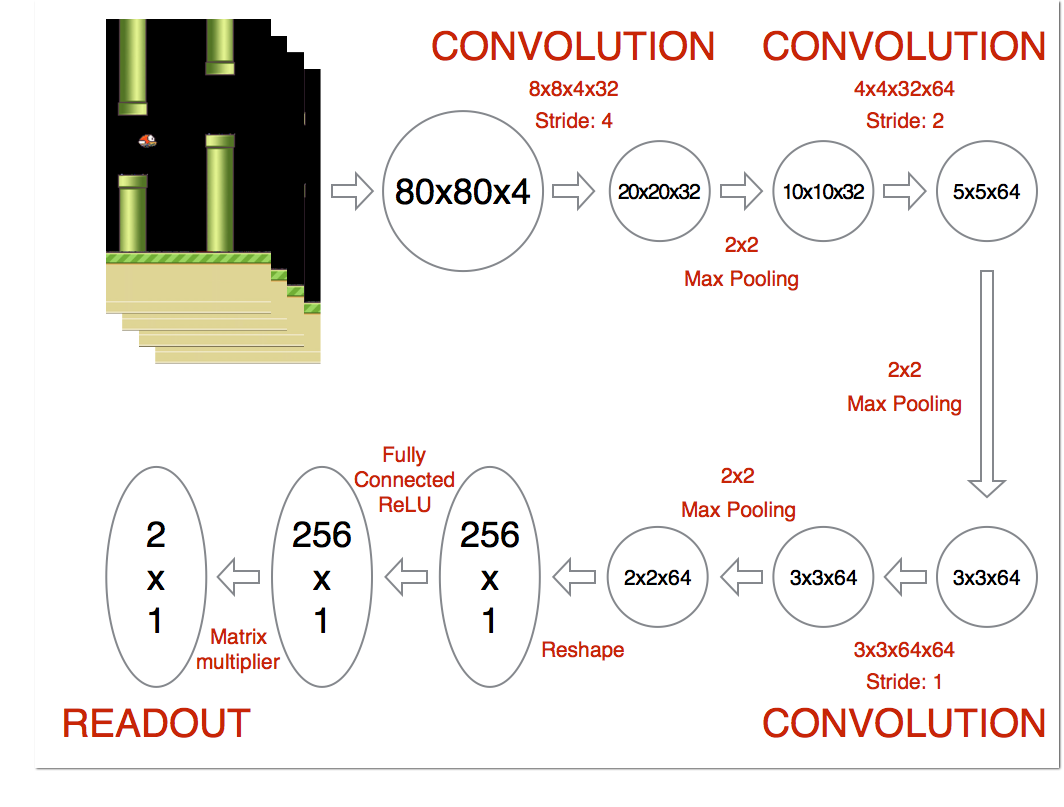
\includegraphics[scale=0.4]{rl_1.png}
	\caption{网络模型.}
	\label{fig:rl_1}
\end{figure}

游戏环境中,单步奖励为$0.1$,越过一个管道$+1$,死亡得到$-1$的惩罚. 可采用其他深度学习框架,如 pytorch、keras 等搭建模型并完成训练代码. DQN算法设置可采用如下配置:
\begin{itemize}
	\item GAMMA = 0.99 \# decay rate of past observations;
	\item OBSERVE = 10000. \# timesteps to observe before training;
	\item EXPLORE = 2000000. \# frames over which to anneal epsilon;
	\item FINAL\_EPSILON = 0.0001 \# final value of epsilon;
	\item INITIAL\_EPSILON = 0.1~0.2 \# starting value of epsilon;
	\item REPLAY\_MEMORY = 50000 \# number of previous transitions to remember;
	\item BATCH = 32 \# size of minibatch;
	\item FRAME\_PER\_ACTION = 1.
\end{itemize}

默认一直训练不会终止,每$10,000$ frames保存一个模型,默认最大保存$5$个,保存的模型可恢复用来测试,默认保存在save\_model 目录下. 采用GPU可加速训练,仅使用双核CPU训练时,采用如上配置,总样本量到$1$M ($1,000,000$个state) 需要时间为$20$~$24$h,大概$3$M可训练出相当不错的策略,考虑到计算咨询和时间,可自行选择训练量.

采用其他深度学习框架时,只需要保持从环境中获得返回的状态、奖励信息,以及是否终止,并可在环境中执行action (再次注意,action为$2$维one-hot编码). Agent与环境交互过程如下所示:
\begin{itemize}
	\item sys.path.append("game/");
	\item import wrapped\_flappy\_bird as game \# import game environment;
	\item game\_state = game.GameState() \# initialize;
	\item \# execute an action and get info from the environment;
	\item $x_t, r_0$, terminal = game\_state.frame\_step(action).
\end{itemize}

本实验提交要求:

仅需提供补全后deep\_q\_network.py文件,以及训练后的短视频 (连续飞行$5-10$s 即可) 或图片或gif动图等辅助证明材料,并说明训练使用样本量. 如果有任何修改或补充说明,请一并说明. (建议写Readme文件或报告)



\begin{mySol}
此处用于写解答(中英文均可)

\end{mySol}
\newpage


\bibliographystyle{plain}
\bibliography{ref}
\end{document}
